%%%%%%%%%%%%%%%%%%%%%%%%%%%%%%%%%%%%%%%%%
% Jacobs Landscape Poster
% LaTeX Template
% Version 1.0 (29/03/13)
%
% Created by:
% Computational Physics and Biophysics Group, Jacobs University
% https://teamwork.jacobs-university.de:8443/confluence/display/CoPandBiG/LaTeX+Poster
% 
% Further modified by:
% Nathaniel Johnston (nathaniel@njohnston.ca)
%
% This template has been downloaded from:
% http://www.LaTeXTemplates.com
%
% License:
% CC BY-NC-SA 3.0 (http://creativecommons.org/licenses/by-nc-sa/3.0/)
%
%%%%%%%%%%%%%%%%%%%%%%%%%%%%%%%%%%%%%%%%%

%----------------------------------------------------------------------------------------
%	PACKAGES AND OTHER DOCUMENT CONFIGURATIONS
%----------------------------------------------------------------------------------------

\documentclass[final]{beamer}

\usepackage[size=a0,scale=1.24]{beamerposter} % Use the beamerposter package for laying out the poster

\usetheme{confposter} % Use the confposter theme supplied with this template

\setbeamercolor{block title}{fg=ngreen,bg=white} % Colors of the block titles
\setbeamercolor{block body}{fg=black,bg=white} % Colors of the body of blocks
\setbeamercolor{block alerted title}{fg=white,bg=dblue!70} % Colors of the highlighted block titles
\setbeamercolor{block alerted body}{fg=black,bg=dblue!10} % Colors of the body of highlighted blocks
% Many more colors are available for use in beamerthemeconfposter.sty

%-----------------------------------------------------------
% Define the column widths and overall poster size
% To set effective sepwid, onecolwid and twocolwid values, first choose how many columns you want and how much separation you want between columns
% In this template, the separation width chosen is 0.024 of the paper width and a 4-column layout
% onecolwid should therefore be (1-(# of columns+1)*sepwid)/# of columns e.g. (1-(4+1)*0.024)/4 = 0.22
% Set twocolwid to be (2*onecolwid)+sepwid = 0.464
% Set threecolwid to be (3*onecolwid)+2*sepwid = 0.708

\newlength{\sepwid}
\newlength{\onecolwid}
\newlength{\twocolwid}
\newlength{\threecolwid}
\setlength{\paperwidth}{48in} % A0 width: 46.8in
\setlength{\paperheight}{36in} % A0 height: 33.1in
\setlength{\sepwid}{0.024\paperwidth} % Separation width (white space) between columns
\setlength{\onecolwid}{0.22\paperwidth} % Width of one column
\setlength{\twocolwid}{0.464\paperwidth} % Width of two columns
\setlength{\threecolwid}{0.708\paperwidth} % Width of three columns
\setlength{\topmargin}{-0.5in} % Reduce the top margin size
%-----------------------------------------------------------

\usepackage{graphbox,graphicx}  % Required for including images

\usepackage{booktabs} % Top and bottom rules for tables

\usepackage{algorithm2e}
\usepackage{amsmath}
\DeclareMathOperator*{\argmax}{argmax}

%----------------------------------------------------------------------------------------
%	TITLE SECTION 
%----------------------------------------------------------------------------------------

\title{Supervised Machine Learning for Extractive Query Based Summarisation of Biomedical Data} % Poster title

\author{Mandeep Kaur \and Diego Moll\'a} % Author(s)

\institute{Macquarie University} % Institution(s)

%----------------------------------------------------------------------------------------

\begin{document}

\addtobeamertemplate{block end}{}{\vspace*{2ex}} % White space under blocks
\addtobeamertemplate{block alerted end}{}{\vspace*{2ex}} % White space under highlighted (alert) blocks

\setlength{\belowcaptionskip}{2ex} % White space under figures
\setlength\belowdisplayshortskip{2ex} % White space under equations

\begin{frame}[t] % The whole poster is enclosed in one beamer frame

\begin{columns}[t] % The whole poster consists of three major columns, the second of which is split into two columns twice - the [t] option aligns each column's content to the top

\begin{column}{\sepwid}\end{column} % Empty spacer column

\begin{column}{\twocolwid} % The first column

%----------------------------------------------------------------------------------------
%	CONTRIBUTIONS
%----------------------------------------------------------------------------------------

\begin{alertblock}{Contributions}
\Large Query-focused multi-document extractive summarisation of biomedical data (data from the BioASQ Challenge):
\begin{enumerate}
\item A comparison between classification and regression approaches.
\item A comparison of annotation methods for classification-based approaches.
\end{enumerate}

\end{alertblock}

%\begin{block}{Introduction}
%\Large
%\begin{itemize}
%    \item We address the task of automatic query-based summarisation of biomedical text by using supervised machine learning techniques.

%\item In addition, this research also deals with a burning issue of availability of annotated corpora for supervised learning. 

%\item We utilised a biomedical corpus provided by the BioASQ Challenge. 

%\item The training data set contains a total of 1306 questions.

%\end{itemize}

%\end{block}


\begin{columns}
\column{\onecolwid}

\begin{block}{\Large Features}
\Large
\begin{itemize}
\item tf-idf vector of the candidate sentence.
\item Cosine similarity between question and candidate sentence.
\end{itemize}
\end{block}

\begin{block}{\Large Data annotation for regression}
\Large F1 ROUGE-SU4 score of the sentence compared to the target summary. 
\end{block}

\begin{block}{\Large Data annotation for classification}
\Large
\begin{enumerate}
\item Label three highest ROUGE-SU4 sentences with~1, the rest with~0.
\item Label all sentences with ROUGE-SU4 $>$ 0.1 with~1, the rest with~0.
\item A variant of the Marcu algorithm.
\end{enumerate}
\end{block}

\column{\onecolwid}
\begin{figure}
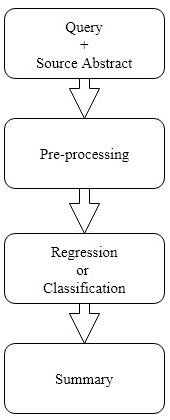
\includegraphics[width=0.6\linewidth]{model.png}
\caption{Summarisation Model\label{fig:model}}
\end{figure}

\end{columns}


\end{column} % End of the second column

\begin{column}{\sepwid}\end{column} % Empty spacer column

\begin{column}{\twocolwid} % The third column

\begin{block}{\Large Marcu annotation}
\large
\begin{algorithm}[H]
\DontPrintSemicolon
\KwData{\\
Abstract ($A$):  The reference summary.\\ 
Text ($T$): Input text to summarise.\\
}
\KwResult{\\
Extract ($E$): A set of sentences from text which has maximum similarity to abstract}
\vspace{1ex}
    \nl $T_1, \cdots\ T_n$ = sentences from $T$\;
    \nl Stem and delete stop words from $A, T_1, \cdots\ T_n$\;
    \nl $E$ = T\;
    \nl $S = \argmax_{S'\in E}Sim(E\backslash S', A)$\;
    \nl \While{$Sim(E,A) < Sim(E\backslash S, A)$}{
                             $E = E\backslash S$\;
                             $S = \argmax_{S'\in E}Sim(E\backslash S', A)$\;}
\caption{The Marcu annotation.\label{algo}}
\end{algorithm}

\vspace{2cm}

\end{block}

%\begin{block}{Results}
%\begin{figure}
%\centering
%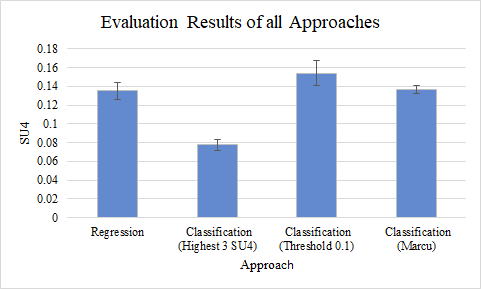
\includegraphics[width=\linewidth]{resultfig_colored.png}
%\caption{Comparison of the results of the regression and three classification approaches. The results show the mean of 10-fold cross-validation, and the error bars show the standard deviation.\label{fig:all_approaches}}
%\end{figure}

%\end{block}

%----------------------------------------------------------------------------------------
%	CONCLUSION
%----------------------------------------------------------------------------------------

\begin{alertblock}{\Large Conclusions}
\Large See the poster!
\end{alertblock}

%----------------------------------------------------------------------------------------
%	CONTACT INFORMATION
%----------------------------------------------------------------------------------------

\setbeamercolor{block alerted title}{fg=black,bg=norange} % Change the alert block title colors
\setbeamercolor{block alerted body}{fg=black,bg=white} % Change the alert block body colors

\vspace{-1cm}

\begin{alertblock}{Contact Information}
\Large\href{http://comp.mq.edu.au/~diego/}{http://comp.mq.edu.au/\~{}diego/}\hfill
\href{mailto:diego.molla-aliod@mq.edu.au}{diego.molla-aliod@mq.edu.au}

\end{alertblock}
%----------------------------------------------------------------------------------------


\includegraphics[align=t,width=0.3\linewidth]{Macquarie.png}
\hfill

\includegraphics[align=t,width=0.3\linewidth]{data61.png}

%----------------------------------------------------------------------------------------
%	ACKNOWLEDGEMENTS
%----------------------------------------------------------------------------------------

%\setbeamercolor{block title}{fg=red,bg=white} % Change the block title color
%\vspace{-3cm}
%\begin{block}{Acknowledgements}

\hfill Research partly funded by CSIRO's Data61
%\end{block}


\end{column} % End of the third column

\end{columns} % End of all the columns in the poster


\end{frame} % End of the enclosing frame

\end{document}
